\documentclass[12pt,a4paper]{article}
\usepackage{fontawesome5}
\usepackage{xcolor}

\usepackage[T1]{fontenc}
\usepackage[utf8]{inputenc}
\usepackage{dsfont} 
\usepackage[polish]{babel}
\usepackage{amsmath}
\usepackage{graphicx}
\usepackage[top=1in, bottom=1.5in, left=1.25in, right=1.25in]{geometry}

\usepackage{subfig}
\usepackage{multirow}
\usepackage{multicol}
\graphicspath{{Images/}}
\usepackage{xcolor,colortbl}
\usepackage{float}
\usepackage{hyperref}
\usepackage{listings}

\newcommand \comment[1]{\textbf{\textcolor{red}{#1}}}

%\usepackage{float}
\usepackage{fancyhdr} % Required for custom headers
\usepackage{lastpage} % Required to determine the last page for the footer
\usepackage{extramarks} % Required for headers and footers
\usepackage{indentfirst}
\usepackage{placeins}
\usepackage{scalefnt}
\usepackage{xcolor,listings}
\usepackage{textcomp}
\usepackage{color}
\usepackage{verbatim}
\usepackage{framed}


\definecolor{codegreen}{rgb}{0,0.6,0}
\definecolor{codegray}{rgb}{0.5,0.5,0.5}
\definecolor{codepurple}{HTML}{C42043}
\definecolor{backcolour}{HTML}{F2F2F2}
\definecolor{bookColor}{cmyk}{0,0,0,0.90}  
\color{bookColor}

\lstset{upquote=true}

\lstdefinestyle{mystyle}{
	backgroundcolor=\color{backcolour},   
	commentstyle=\color{codegreen},
	keywordstyle=\color{codepurple},
	numberstyle=\numberstyle,
	stringstyle=\color{codepurple},
	basicstyle=\footnotesize\ttfamily,
	breakatwhitespace=false,
	breaklines=true,
	captionpos=b,
	keepspaces=true,
	numbers=left,
	numbersep=10pt,
	showspaces=false,
	showstringspaces=false,
	showtabs=false,
}
\lstset{style=mystyle}

\newcommand\numberstyle[1]{%
	\footnotesize
	\color{codegray}%
	\ttfamily
	\ifnum#1<10 0\fi#1 |%
}

\definecolor{shadecolor}{HTML}{F2F2F2}

\newenvironment{sqltable}%
{\snugshade\verbatim}%
{\endverbatim\endsnugshade}

% Margins
\addtolength{\footskip}{0cm}
\addtolength{\textwidth}{1.4cm}
\addtolength{\oddsidemargin}{-.7cm}

\addtolength{\textheight}{1.6cm}
%\addtolength{\topmargin}{-2cm}

% paragrafo
\addtolength{\parskip}{.2cm}

% Set up the header and footer
\pagestyle{fancy}
\lhead{\hmwkClass: \hmwkTitle} % Top center header
\rhead{\firstxmark} % Top right header
\lfoot{Maria Koren} % Bottom left footer
\cfoot{} % Bottom center footer
\rfoot{} % Bottom right footer
\renewcommand{\headrulewidth}{1pt}
\renewcommand{\footrulewidth}{1pt}

    
\newcommand{\hmwkTitle}{Analiza danych użytkowników social media} 
\newcommand{\hmwkDueDate}{\today} 
\newcommand{\hmwkClass}{Inteligencja Obliczeniowa}
\newcommand{\hmwkAuthorName}{Maria Koren}

% trabalho 
\begin{document}
% capa
\begin{titlepage}
    \vfill
	\begin{center}
	\hspace*{-1cm}
	\vspace*{0.5cm}
    \includegraphics[scale=0.55]{images/loga.png}\\
	\textbf{Uniwersytet Gdański \\ [0.05cm]Wydział Matematyki, Fizyki i Informatyki \\ [0.05cm] Instytut Informatyki}

	\vspace{0.6cm}
	\vspace{4cm}
	{\huge \textbf{\hmwkTitle}}\vspace{8mm}
	
	{\large \textbf{\hmwkAuthorName}}\\[3cm]
	
		\hspace{.45\textwidth} %posiciona a minipage
	   \begin{minipage}{.5\textwidth}

	  \end{minipage}
	  \vfill
	%\vspace{2cm}
	
	\textbf{Gdańsk}
	
	\textbf{\hmwkDueDate}
	\end{center}
	
\end{titlepage}

\newpage
\setcounter{secnumdepth}{5}
\tableofcontents
\newpage

\section{Wstęp}

Została przeprowadzona analiza danych użytkowników social media na podstawie bazy danych \href{https://www.kaggle.com/datasets/arindamsahoo/social-media-users/data}{link}.W celu analizy najpierw wykonano preprocessing danych, klasyfikacja prostymi klasyfikatorami, klasyfikacja sieciami neuronowymi. Oraz wyszukano reguły asocjacyjne.

\newpage

\section{Preprocessing}

\subsection{Znaczenia kolumn, problemy w bazie}
Główne zadania preprocessingu umieszczone w pliku \textit{main.py}. 

Baza danych \textit{SocialMediaUsersDataset.csv} zawiera następujące kolumny: UserID, Name, Gender, DOB, Interests, City, Country. 

Dla dalszej analizy kolumny UserId oraz Name usunięte, ponieważ nie wnoszą żadnych informacji. I została zapisana do pliku \textit{DataWithNoNameNoId.csv}.

Nastęnie kolumne DOB, przechowująca daty urodzenia użytkowników przerobiono na kolumne Age, gdzie jest wiek. 

Zatem kolumnę Gender, która przechowuje dane o płci w postaci słów "Male" oraz "Female" zmapowano na 0 oraz 1 w następujący sposób:

\begin{lstlisting}[language=Python]
gender_mapping = {'Male': 0, 'Female': 1}
df['Gender'] = df['Gender'].map(gender_mapping)
\end{lstlisting}

Jednym z największych problemów w tej bazie są kraje oraz miasta. Ponieważ ilość wystąpień każdego kraju jest dość różna. Na przykład najczęściej się pojawia 'United States' 12311 razy, a najmniej 'Saint Lucia', 'American Samoa', 'Saint Martin' pojawiają się jednen raz. Z miastami jest trudniej, ponieważ one są powiązane z krajami. Dlatego przyjęte było następujące podejście: usunąć kolumnę 'City'.A dla krajów wybrano 10 z nich najczęście występujących.

Drugim dużym problemem w bazie była kolumna 'Interests', reprezentująca zainteresowania osób. Problemem w tej kolumnie jest to, że może ona zawierać w sobie jak zarówno jedno zainteresowanie, jak i kilka z nich. Również występował problem, że zaiteresowanie 'Fashion' było blisko 18 000 razy, a reszta około 9 000. Więc do finalnej bazy wybrano 9 najczęstszych z wyjątkiem 'Fashion'.

Z uwagi na małą ilość kolumn w bazie dodano jeszcze kolumnę InterestCount, reprezentującą ilość zainteresowań danej osoby.

\newpage

\subsection{Finalna Baza}
Finalna baza zawiera w sobie kolumny tylko liczbowe, co ułatwia przetwarzanie danych. Kolumny to: "Gender, Interests, Country, InterestCount, Age". Każde zainteresowanie oraz kraj zostały zmapowane na liczby. Przy czym dla każdego zainteresowania wystęuje równa ilość rekordów dla każdego kraju, zrobiono to w celu zbalansowania bazy danych. Takie zestawienie bazy danych daje łącznie 6 300 rekordów w bazie \textit{data.csv}.

\begin{lstlisting}[language=Python]
selected_countries = ['United States', 'India', 'China', 'Brazil', 'Russia', 'Germany', 'Japan', 'United Kingdom', 'France', 'Mexico']
selected_interests = ["'Cooking'", "'Pets'" ,"'Movies'" ,"'Gaming'", "'Fitness'" ,"'Outdoor activities'", "'Travel'", "'Business and entrepreneurship'" , "'Social causes and activism'"]

country_to_index = {country: index for index, country in enumerate(selected_countries)}
interest_to_index = {interest: index for index, interest in enumerate(selected_interests)}

df['Country'] = df['Country'].apply(lambda x: country_to_index[x] if x in selected_countries else None)
df = df.dropna(subset=['Country']).astype({'Country': 'int'})
df = df[df['Interests'].isin(selected_interests)]
df['Interests'] = df['Interests'].apply(lambda x: interest_to_index[x] if x in selected_interests else None)
df = df.dropna(subset=['Interests']).astype({'Interests': 'int'})

final_df = pd.DataFrame(columns=df.columns)
grouped = df.groupby(['Country', 'Interests'])
for (country, interest), data in grouped:
    if len(data) < 70:
        final_df = pd.concat([final_df, data], ignore_index=True)
    else:
        sampled_data = data.sample(n=70, random_state=42)
        final_df = pd.concat([final_df, sampled_data], ignore_index=True)

final_df = final_df.groupby(['Country', 'Interests']).head(70).reset_index(drop=True)

final_df.to_csv('data.csv', index=False)
\end{lstlisting}
Również jako preprocessing wykonano skalowanie danych w kolumnach InterestCount i Age, plik \textit{scaled.py}. Skalowana baza danych jest zapisana do pliku \textit{data\textunderscore scaled.csv}

\newpage

\section{Klasyfikacja prostymi klasyfikatorami}

\subsection{Klasyfikacja zainteresowań}

Wykonano klasyfikację prostymi klasyfikatorami poznanymi na zajęciach: 

\begin{enumerate}
    \item Nearest Neighbor (3, 5, 11, 100)
    \item Naive Bayes
    \item Desicion Tree
\end{enumerate}

Oraz na klasyfikatorze, znalezionym samodzielnie: Random Forest (łączy w sobie kilka drzew decyzyjnych).

Za pomocą wyżej wymienionych klasyfikatorów najpierw klasyfikałam zainteresowania. Na bazie danych bez skalowania wyszły takie wyniki:

\begin{itemize}
    \item Dokładność klasyfikatora 3-NN: 0.12163839470417874
    \item Dokładność klasyfikatora 5-NN: 0.10881257757550683
    \item Dokładność klasyfikatora 11-NN: 0.11170872983036823
    \item Dokładność klasyfikatora 100-NN: 0.11170872983036823
    \item Dokładność klasyfikatora Naive Bayes: 0.1119155978485726
    \item Dokładność klasyfikatora Random Forest: 0.11005378568473315
    \item Dokładność klasyfikatora Desicion Tree: 0.11605295821266032
\end{itemize}

\begin{figure}[h]
    \centering
    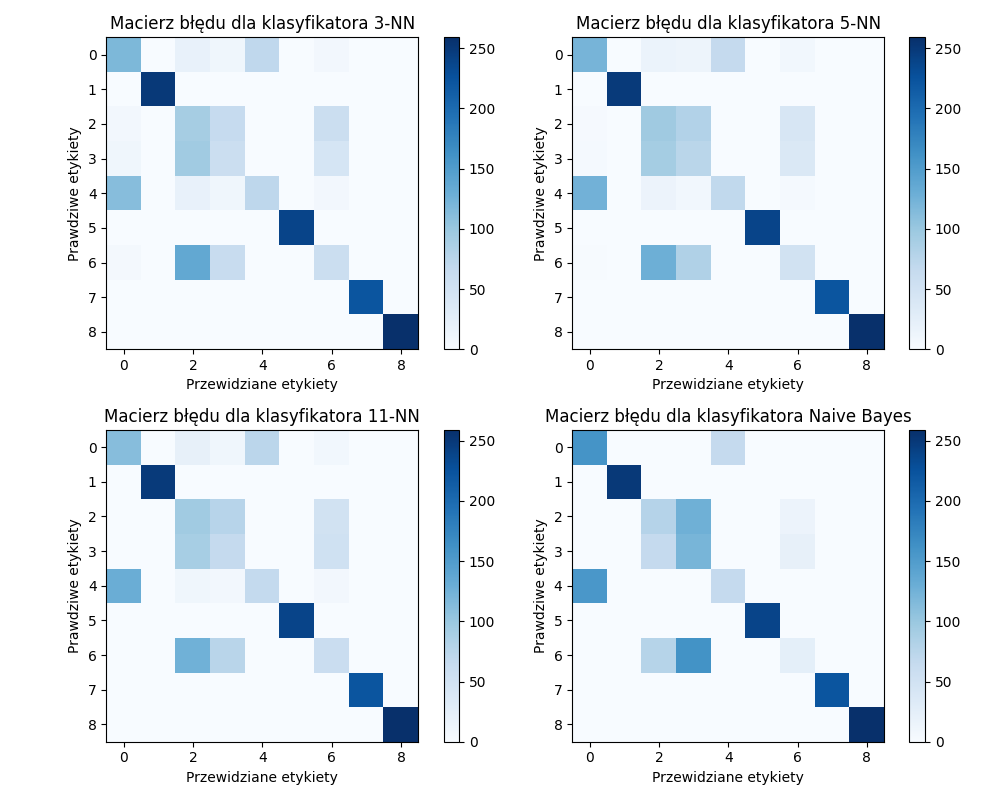
\includegraphics[width=10cm]{images/macierze_bledow.png}
    \caption{Proste klasyfikatore na bazie bez skalowania}
    \label{fig:pk}
\end{figure}

Na bazie ze skalowaniem wyniki wyszły następujące:

\begin{itemize}
    \item Dokładność klasyfikatora 3-NN: 0.12246586677699628
    \item Dokładność klasyfikatora 5-NN: 0.11708729830368225
    \item Dokładność klasyfikatora 11-NN: 0.112122465866777
    \item Dokładność klasyfikatora 100-NN: 0.112122465866777
    \item Dokładność klasyfikatora Naive Bayes: 0.1119155978485726
    \item Dokładność klasyfikatora Random Forest: 0.10819197352089367
    \item Dokładność klasyfikatora Desicion Tree: 0.11563922217625155
\end{itemize}

\begin{figure}[h]
    \centering
    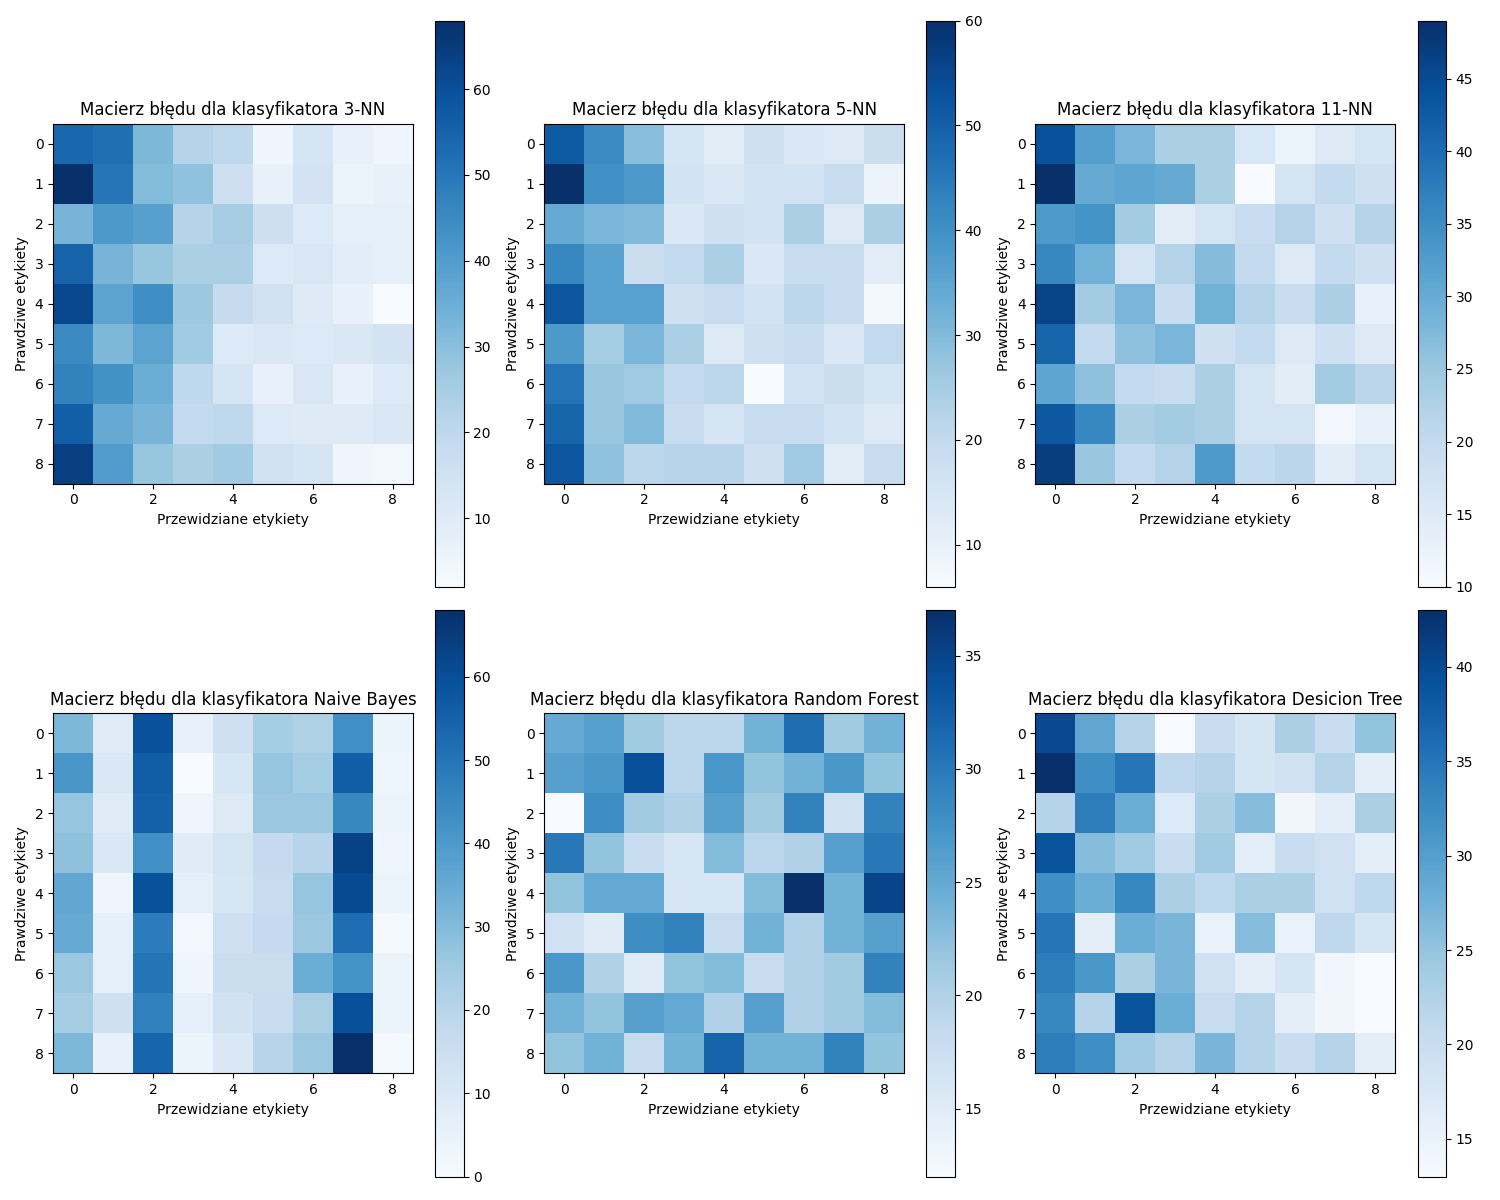
\includegraphics[width=10cm]{images/macierze_bledow_scaled.png}
    \caption{Proste klasyfikatore na bazie ze skalowaniem}
    \label{fig:pk1}
\end{figure}


Dla klasyfikatorów najbliższych sąsiadów lepsze wyniki dała baza ze skalowaniem, natomiast dla Random Forest oraz Desicion Tree baza bez skalowania daje lepsze wyniki. W każdym z przypadków lepsze wyniki dał klasyfikator 3NN.

\textbf{Podsumowanie}. Ponieważ jest 9 klas, prawdopodobieństwo losowego trafiania w poprawne zainteresowanie wynosi 0.11, można wnioskować że te klasyfikatory poradziły sobie trochę lepiej niż zwykłe losowanie.

\newpage

\subsection{Klasyfikacja płci}

Kolejną rzeczą którą sklasyfikowałam za pomocą prostych klasyfikatorów jest klasyfikacja płci.

Na bazie danych bez skalowania wyszły takie wyniki:

\begin{itemize}
    \item Dokładność klasyfikatora 3-NN: 0.4888291270169632
    \item Dokładność klasyfikatora 5-NN: 0.49296648738105087
    \item Dokładność klasyfikatora 11-NN: 0.5066197765825403
    \item Dokładność klasyfikatora 100-NN: 0.5066197765825403
    \item Dokładność klasyfikatora Naive Bayes: 0.49007033512618947
    \item Dokładność klasyfikatora Random Forest: 0.4927596193628465
    \item Dokładność klasyfikatora Desicion Tree: 0.49958626396359124
\end{itemize}

\begin{figure}[h]
    \centering
    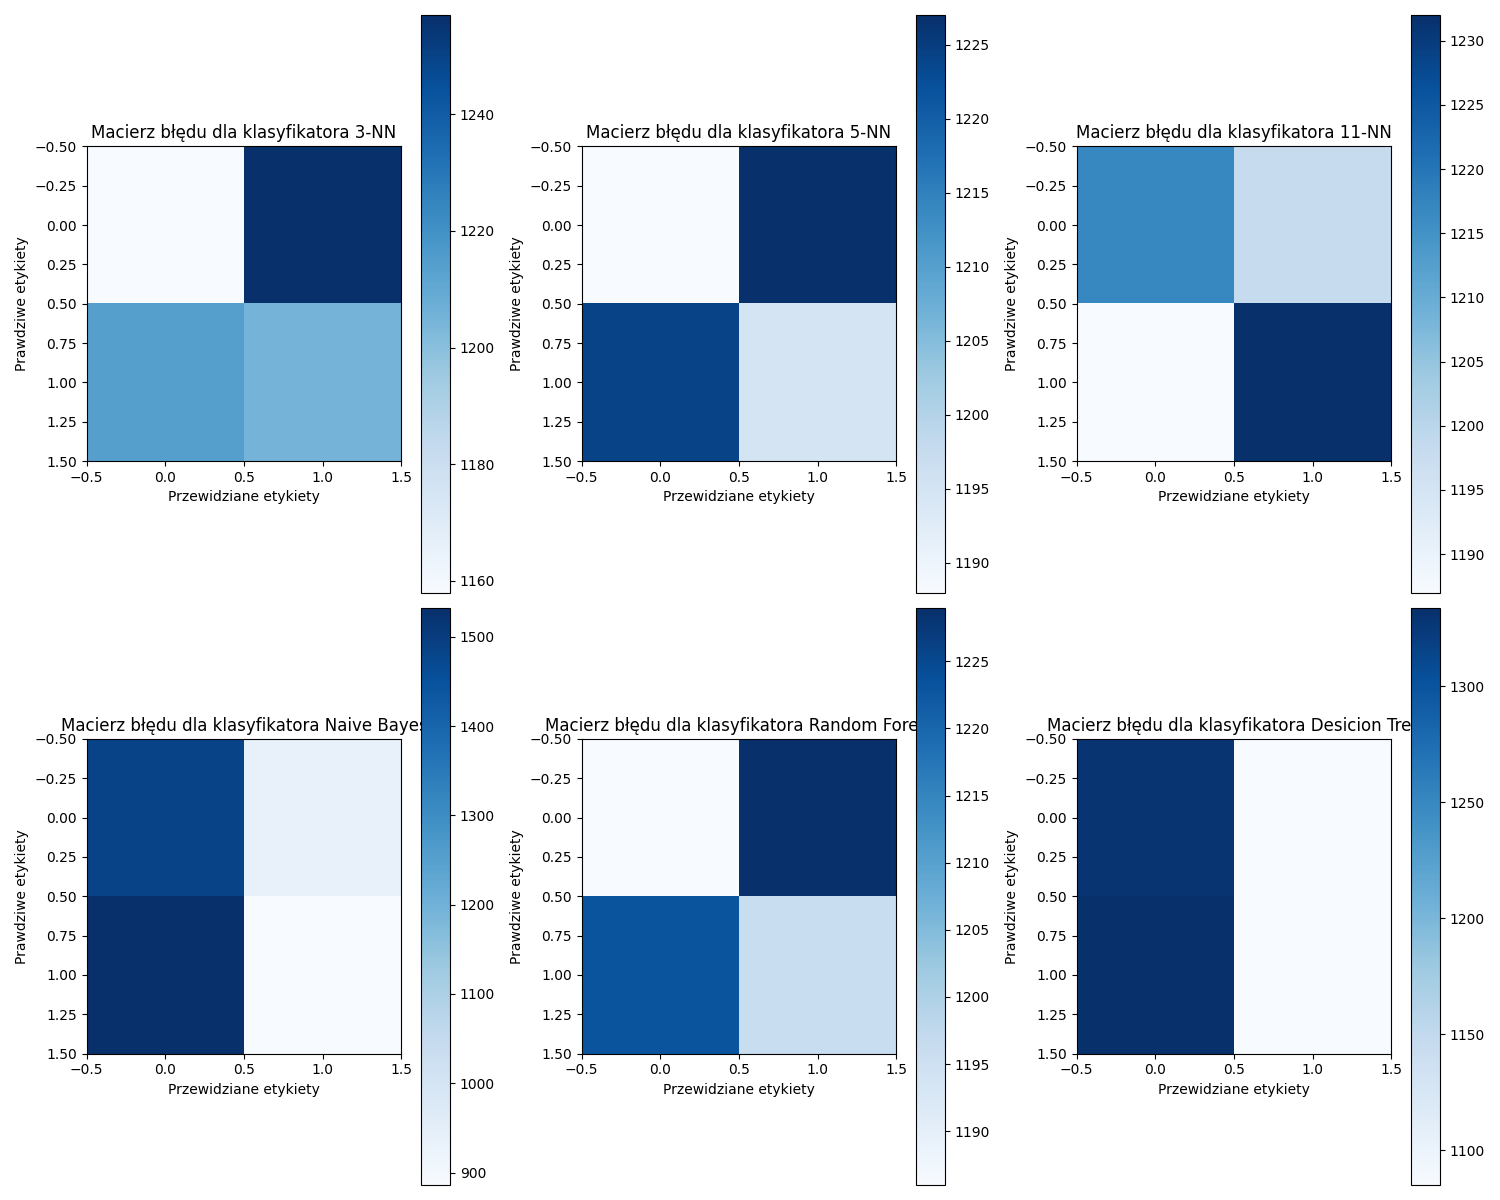
\includegraphics[width=10cm]{images/macierze_bledow_gender.png}
    \caption{Proste klasyfikatore na bazie bez skalowania}
    \label{fig:pk2}
\end{figure}

Na bazie ze skalowaniem wyniki wyszły następujące:

\begin{itemize}
    \item Dokładność klasyfikatora 3-NN: 0.49813818783616054
    \item Dokładność klasyfikatora 5-NN: 0.49089780719900705
    \item Dokładność klasyfikatora 11-NN: 0.4931733553992553
    \item Dokładność klasyfikatora 100-NN: 0.4931733553992553
    \item Dokładność klasyfikatora Naive Bayes: 0.49007033512618947
    \item Dokładność klasyfikatora Random Forest: 0.4902772031443939
    \item Dokładność klasyfikatora Desicion Tree: 0.49793131981795613
\end{itemize}

\begin{figure}[h]
    \centering
    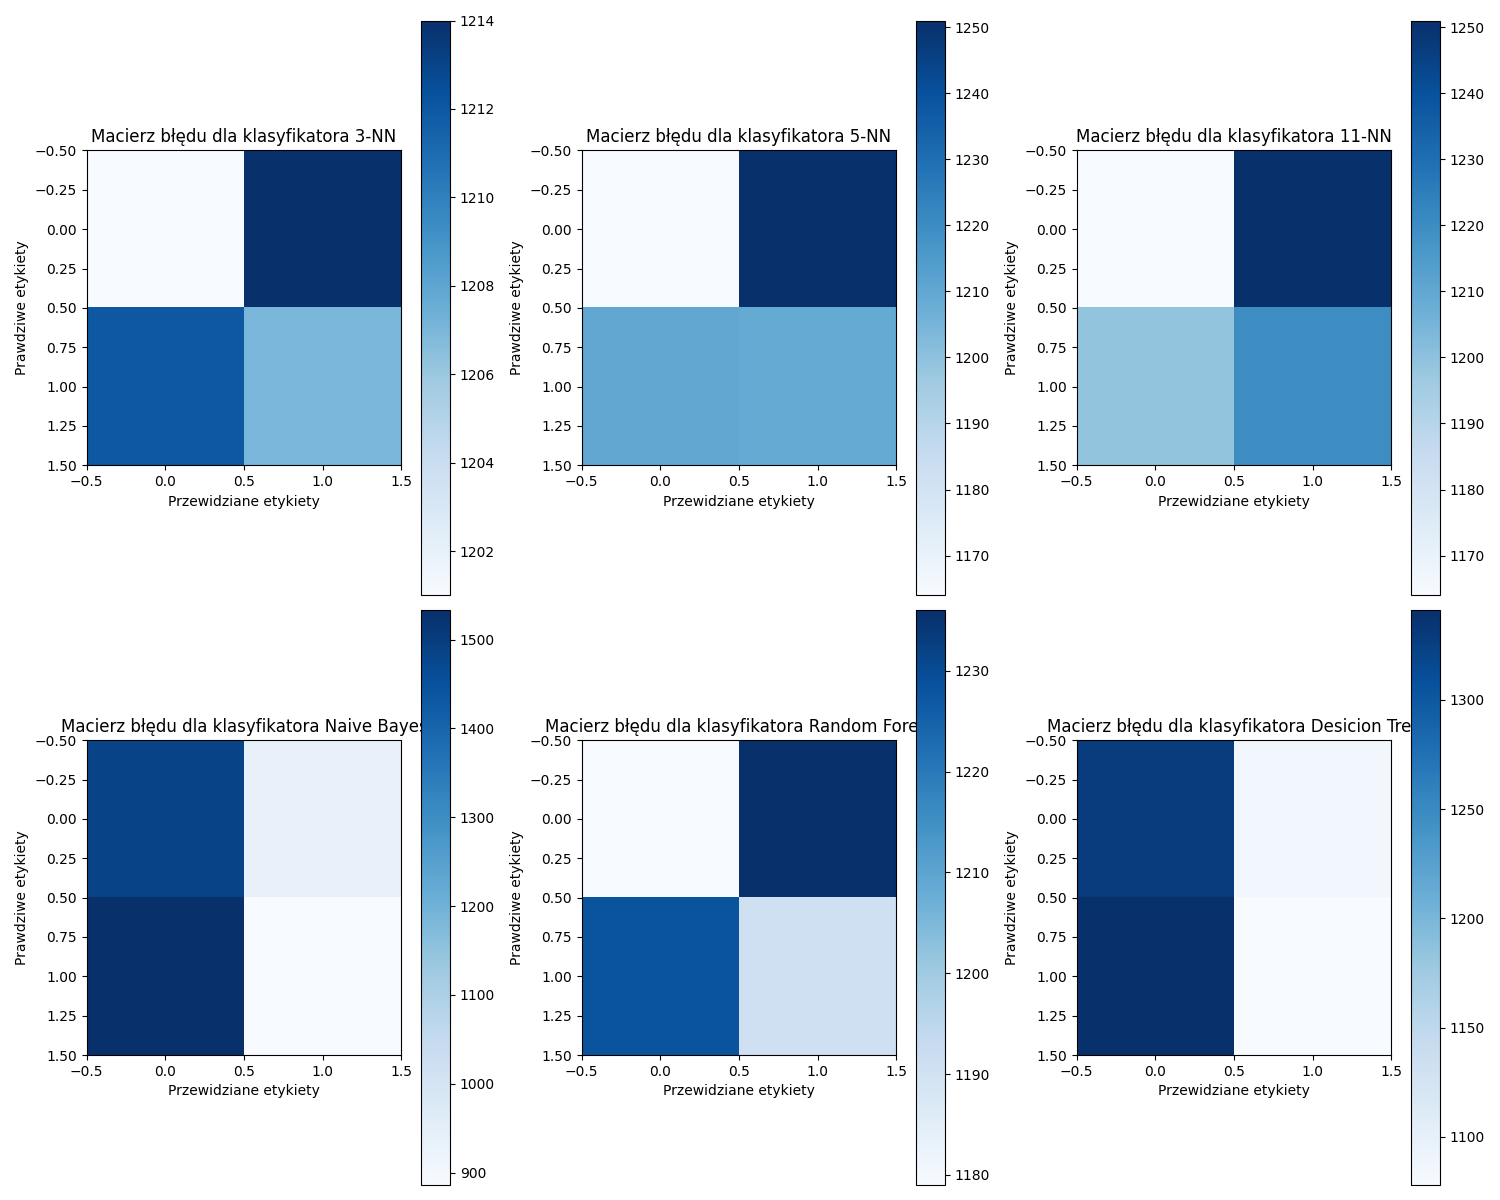
\includegraphics[width=10cm]{images/macierze_bledow_gender_scaled.png}
    \caption{Proste klasyfikatore na bazie ze skalowaniem}
    \label{fig:pk3}
\end{figure}

Wnioski odnośnie skalowania danych takie, jak poprzednio.

\textbf{Podsumowanie}. Ponieważ klas jest tylko 2, to prawdopodobieństwo losowego trafiania w poprawne zainteresowanie wynosi 0.5. Więc można wnioskować, że proste klasyfikatory w tym przykładzie poradziły sobie gorzej niż losowanie. Trochę lepsze wyniki dali 11NN oraz 100NN na bazie bez skalowania.

\newpage

\section{Klasyfikacja sieciami neuronowymi}

Za pomocą sieci neuronowych sklasyfikowano 2 opcje:

\begin{enumerate}
    \item Klasyfikacja zainteresowań (plik \textit{nn.py})
    \item Klasyfikacja krajów (plik \textit{nn2.py})
\end{enumerate}

\subsection{Klasyfikacja zainteresowań}
W wersji ostatecznej została użyta taka sieć:

\begin{lstlisting}[language=Python]
model = Sequential([
    Dense(64, activation='tanh', input_shape=(X_train.shape[1],)),
    Dense(32, activation='tanh'),
    Dense(len(np.unique(y_train)), activation='softmax')
])
\end{lstlisting}

Przed zostawieniem tego modelu były użyte inne sieci, zmieniono ilość warstw, funkcję aktywacyjną. Ale najlepsze wyniki, choć nie o wiele, pokazała właśnie ta sieć. Sieć została wytrenowana na 1000 epokach.

Dokładność tej sieci: $12,12\%$.

\begin{figure}[h]
    \centering
    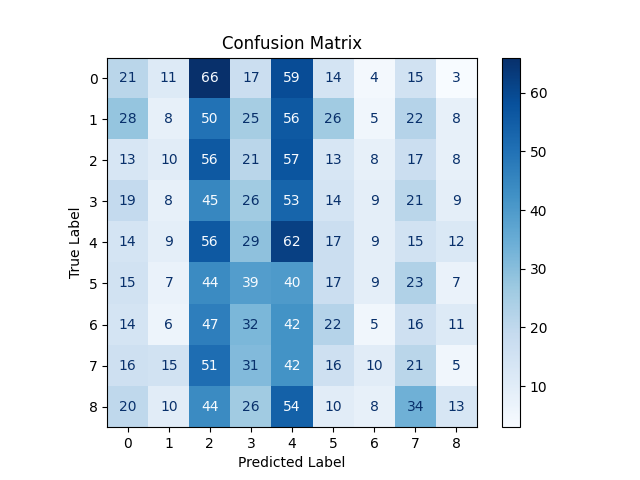
\includegraphics[width=10cm]{images/confusion_matrix_interest.png}
    \caption{Macierz błedów}
    \label{fig:cm_int}
\end{figure}

\subsection{Klasyfikacja krajów}
W wersji ostatecznej została użyta taka sieć:

\begin{lstlisting}[language=Python]
model = Sequential([
    Dense(64, activation='relu', input_shape=(X_train.shape[1],)),
    Dense(32, activation='relu'),
    Dense(len(np.unique(y_train)), activation='softmax')
])

\end{lstlisting}

Przed zostawieniem tego modelu były użyte inne sieci, zmieniono ilość warstw i funkcji aktywacyjne. Ale najlepsze wyniki, choć nie o wiele pokazała właśnie ta sieć. Sieć została wytrenowana na 5000 epokach.

Dokładność tej sieci: $10,01\%$.

\begin{figure}[h]
    \centering
    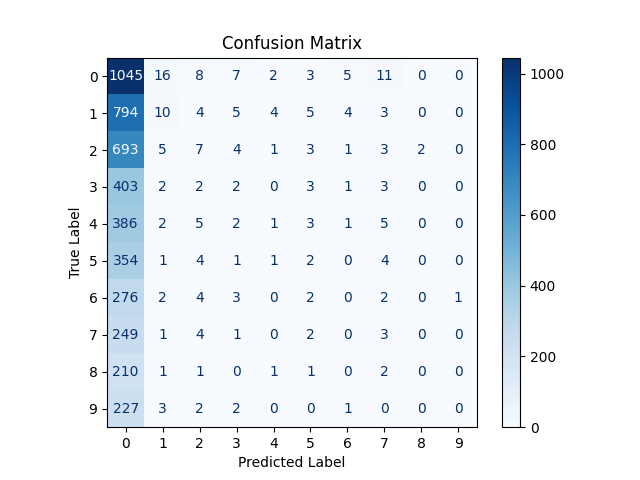
\includegraphics[width=10cm]{images/confusion_matrix_country.png}
    \caption{Macierz błedów}
    \label{fig:cm_c}
\end{figure}

\newpage

\section{Reguły asocjacyjne}

\subsection{Reguły zainteresowań}

Reguły asocjacyjne zostały zbadane odnośnie zainteresowań. Najpierw na pliku oryginalnym zrobiony był dataframe, gdzie kolumny to unikalne zainteresowania, a w wierszch stoją 0 jeżeli zainteresowanie nie wystepuje u danej osoby, 1 jeżeli występuje. Na danych oryginalnych reguły w skrócie można było reprezentować w ten sposób: "Jeżeli interesujesz się czym kolwiek, prawdopodobnie będzisz się interesował Fashion". To wychodziło z powodu mocno niezbalansowanej bazy, o czym było napisane w części o preprocessingu.

Zatem wykonano inny preprocessing: usunięto wszystkie rekordy, zawierające 'Fashion', i powórzono eksperyment. Wyszła 1 reguła: 

\begin{figure}[h]
    \centering
    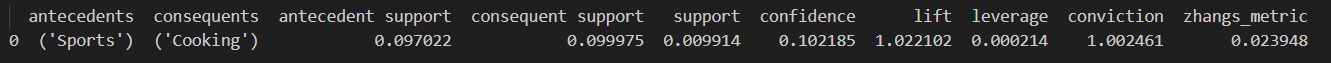
\includegraphics[width=15cm]{images/reguly.png}
    \caption{Reguła zainteresowań}
    \label{fig:reg1}
\end{figure}

Reguła ta oznacza: "Jeżeli interesujesz się sportem, z prawdopodobieństwem 0.097 będziesz się interesował gotowaniem".

\subsection{Inne reguły}

Ponieważ funkcji reguł asocjacyjnych wymagają tylko wartości 0/1 bądź True/False, dla pliku \textit{data.csv} jest potrzebny dalszy preprocessing. W nim usunięto kolumny Interests oraz Country. Dla kolumn Age oraz InterestCount wyliczono średnie znaczenia, wartości poniżej średniej zamieniono na 0, powyżej na 1. Średnia dla wieku jest 44,33, dla zainteresowań 3. Dla przypomnienia, w kolumnie Gender: Male - 0, Female - 1. Wyszły takie reguły:

\begin{figure}[h]
    \centering
    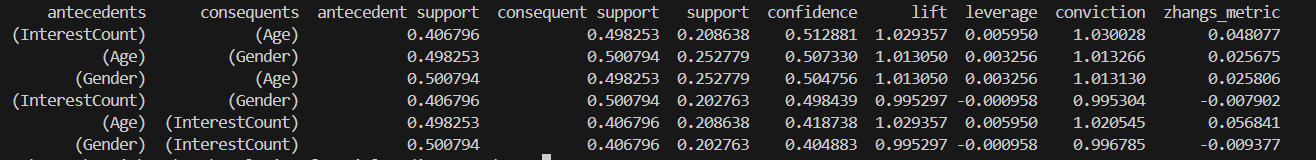
\includegraphics[width=15cm]{images/reguly2.png}
    \caption{Inne reguły}
    \label{fig:reg1}
\end{figure}

Opis reguł:

\begin{enumerate}
    \item Jeżeli masz powyżej 3 zainteresowań, raczej jesteś w wieku powyżej 44 lat
    \item Jeżeli jesteś w wieku powyżej 44 lat, raczej jesteś kobietą.
    \item Jeżeli jesteś kobietą, raczej masz powyżej 44 lat.
    \item Jeżeli masz powyżesz 3 zainteresowań, raczej jesteś kobietą.
    \item Jeżeli masz powużej 44 lat, raczej masz więcej trzech zainteresowań.
    \item Jeżeli jesteś kobietą, raczej masz powyżej 3 zainteresowań.
\end{enumerate}

\newpage

\section{Podsumowanie}

W pracy przeprowadzono analizę danych użytkowników social media. Skorzystano zarówno s prostych klasyfikatorów, jak i sieci neuronowych, będących bardziej złożonym klasyfikatorem.

Fakt, że wynik każdego z klasyfikatoru jest blisko prawdobodobieństwa losowego "strzelania" można wytłumaczyć tym, że analizowane dane mają słabe zależności. To oznacza, że w rzeczywistym świecie trudno zrobić predykcję o zainteresowaniach, na podstawie płci, wieku, miejsca zamieszkania, co zmniejsza szanse na dyskryminację. Również trudno na podstawie zainteresowań, płci i wieku wywnioskować o miejscu zamieszkania, co dodatkowo zmniejsza szansę na dyskryminację.

\end{document}